\section{Neutron Detection}
\subsection{General Remarks}
\begin{itemize}
    \item Neutrons are charge-neutral particles; they can only interact via the strong force and ionize via secondary reactions.
    \item Most neutron detectors consist of a material that converts neutrons into charged particles within a conventional detector.
    \item There are 2 classes of interactions:
    \begin{enumerate}
        \item Slow neutrons (thermal and epithermal), E $<$ 1 keV:\\
        (n,$\gamma$), (n,p), (n,$\alpha$), (n,f)
        \item Fast neutrons, E $>$ 1 keV:\\
        (n,n), (n,n'), (n,xn), (n,xpn), (n,f)
    \end{enumerate}
\end{itemize}
\subsection{Slow Neutron Detection}
\subsubsection{Commonly Used Neutron Reactions}
\begin{itemize}
    \item Commonly used reactions include:
    \begin{itemize}
        \item (n,p):
        \begin{itemize}
            \item[] n $+$ $^3$He $\rightarrow$ p $+$ $^3$H, Q $=$ 0.764 MeV
        \end{itemize}
        \item (n,$\alpha$):
        \begin{itemize}
            \item[] n $+$ $^6$Li $\rightarrow$ $^4$He $+$ $^3$H, Q $=$ 4.78 MeV
            \item[] n $+$ $^{10}$B $\rightarrow$ $^{4}$He $+$ $^7$Li*, Q $=$ 2.31 MeV (94\%)
            \item[] n $+$ $^{10}$B $\rightarrow$ $^{4}$He $+$ $^7$Li, Q $=$ 2.79 MeV (6\%)
        \end{itemize}
        \item (n,$\gamma$): $\sigma\propto1/v$
        \begin{itemize}
            \item[] n $+$ $^{113}$Cd $\rightarrow$ $^{114}$Cd $+$ $\gamma$, Q $\sim$ 8 MeV
            \item[] n $+$ $^{157}$Gd $\rightarrow$ $^{158}$Gd $+$ $\gamma$, Q $\sim$ 8 MeV
        \end{itemize}
        \item (n,f):
        \begin{itemize}
            \item[] n $+$ $^{235}$U $\rightarrow$ fission fragments, Q $\sim$ 200 MeV
        \end{itemize}
    \end{itemize}
\end{itemize}

\subsubsection{The He-3 Proportional Counter}
\begin{itemize}
    \item n $+$ $^3$He $\rightarrow$ p $+$ $^3$H, Q $=$ 764 keV
    \item Assuming E$_n\ll$ Q, with momentum conservation, E$_p=\frac{m_t}{m_p+m_t}$Q $=$ 573 keV, E$_t=\frac{m_p}{m_p+m_t}$Q $=$ 191 keV.
    \item The wall effect, as shown in figure~\ref{fig:He3_wall_effect}, occurs as the proton or triton may escape without detection. The wall effect depends on the tube dimensions and gas pressure. Methods to decrease the wall effect include:
    \begin{itemize}
        \item Building a counter with a diameter as large as possible
        \item Reducing the range of charged particles in $^3$He ($\sim$mm) by increasing gas pressure
        \item Reducing the range of charged particles by adding a small amount of a heavier gas
    \end{itemize} 
\end{itemize}
\begin{figure}[ht]
    \centering
    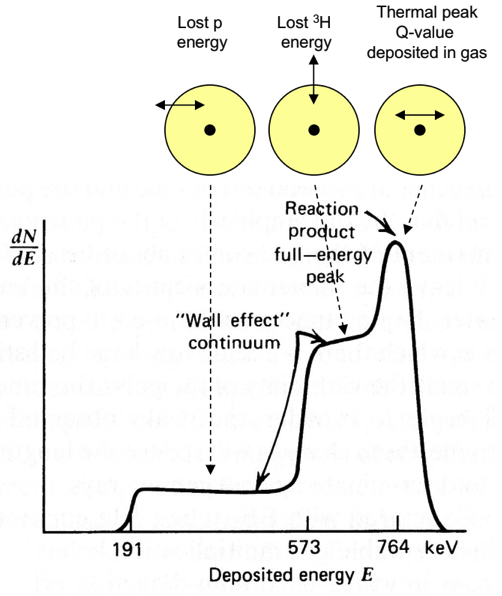
\includegraphics[width=0.4\textwidth]{images/He3_wall_effect.png}
    \caption{Wall effect in the $^3$He proportional counter.}
    \label{fig:He3_wall_effect}
\end{figure}
\subsubsection{The BF3 Slow Neutron Detector}
\begin{figure}[ht]
    \centering
    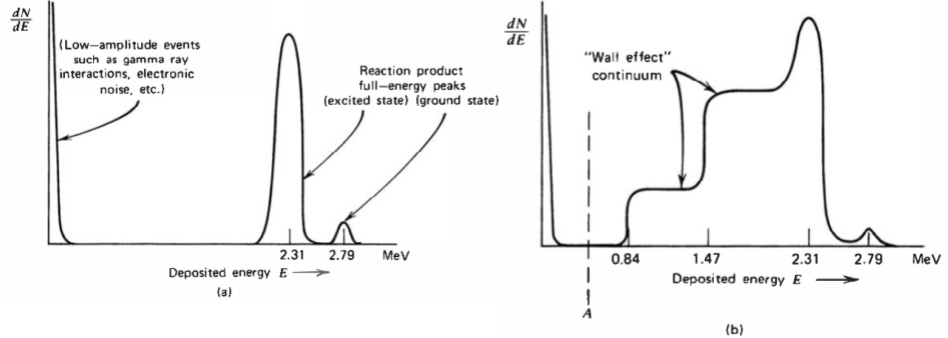
\includegraphics[width=0.8\textwidth]{images/BF3_wall_effect.png}
    \caption{The (a) ideal spectrum and (b) the wall effect in a BF$_3$ proportional tube.}
    \label{fig:BF3_wall_effect}
\end{figure}
\begin{itemize}
    \item n $+$ $^{10}$B $\rightarrow$ $^{4}$He $+$ $^7$Li*, Q $=$ 2.31 MeV (94\%)\\
          n $+$ $^{10}$B $\rightarrow$ $^{4}$He $+$ $^7$Li, Q $=$ 2.79 MeV (6\%)
    \item The BF$_3$ gas is enriched to $>$90\% $^{10}$B
    \item Operated as a proportional or GM counter
    \item To reduce the effects of recombination and negative ion formation, the gas pressure is kept below 1 atm (range of $\alpha$ $\sim$10 mm), leading to pronounced wall effect, as shown in figure~\ref{fig:BF3_wall_effect}.
    \item As in the case of the $^3$He counter, the spectrum reflects the response of the detector, $\emph{not}$ neutron energy. 
    \item BF$_3$ tubes can discriminate against low fluxes of gamma-rays; due to the low stopping power of the secondary electrons created via the interaction of gammas with the detector wall, only a small amount of energy will be deposited, leading to the low-amplitude pulses left to point A in figure~\ref{fig:BF3_wall_effect}(b).
\end{itemize}

\subsubsection{Fission Counters}
\begin{figure}[ht]
    \centering
    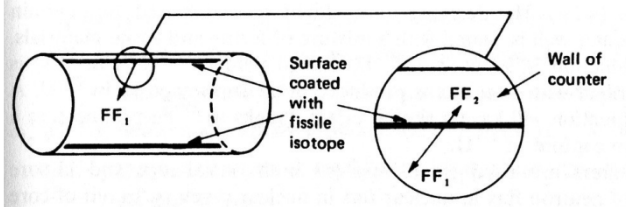
\includegraphics[width=0.4\textwidth]{images/fission_counter_config.png}
    \caption{Configuration of fission counters.}
    \label{fig:fission_counter_config}
\end{figure}
\begin{itemize}
    \item The most common form of fission detectors is an ionization chamber (or proportional counter) that has its inner surfaces coated with a fissile deposit, as shown in figure~\ref{fig:fission_counter_config}.
    \item A large amount of energy is released in each fission reaction ($\sim$200 MeV), with $\sim$160 MeV as the kinetic energy of fission fragments. Therefore, extremely low background rates can be achieved, and neutron counting can be performed with very low count rates. 
    \item Due to the non-linearities for densely ionizing particles (fission fragments), the detector pulses may not be as large as would be calculated based on simple linearity with energy, reducing discrimination capabilities.
    \item Alpha-decay of the fissile deposit creates a continuous background. 
    \item Efficiency of the counter can be increased by increasing the thickness of the deposit, but at the expense of quantitative measurement capabilities. As shown in figure~\ref{fig:fission_counter_efficiency}, while increasing thickness increases detection efficiency, the energy loss of fragments within the deposit will reduce the average fragment energy and distort the shape of the distribution. 
\end{itemize}
\begin{figure}[ht]
    \centering
    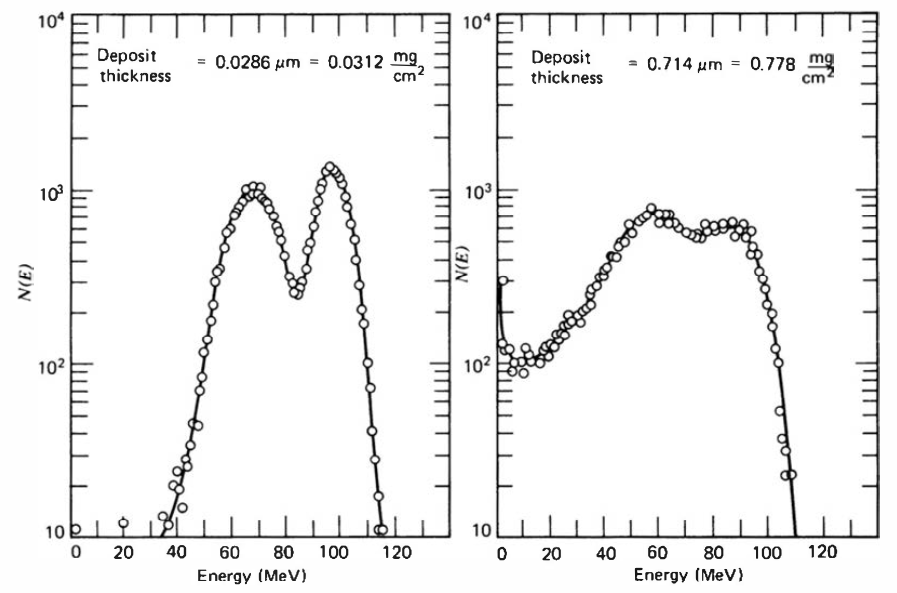
\includegraphics[width=0.6\textwidth]{images/fission_counter_efficiency.png}
    \caption{Energy spectra of fission counters with a thin layer (left) and a thicker layer (right) of fissile deposit.}
    \label{fig:fission_counter_efficiency}
\end{figure}
\subsubsection{Li-Based Scintillators}
\begin{itemize}
    \item n $+$ $^6$Li $\rightarrow$ $^4$He $+$ $^3$H, Q $=$ 4.78 MeV
    \item While there are no Li containing gas available, we have solid LiI(Eu) detectors, similar to NaI(Tl) detectors.
    \item Since the range of reaction products are shorter than dimensions of the detector, there is no wall effect; a single peak will be seen on the spectrum.
    \item The gamma rejection capabilities are inferior to gas-filled detectors; there is a continuous gamma background. (A 4.1 MeV electron will yield about the same light as the 4.78 MeV neutron induced reaction products.)
    \item $^6$Li-glass can be implemented as meters-long fibers, and is capable of fast neutron detection as well. 
    \item Liquid Li-based scintillators allows neutron-gamma pulse-shape discrimination.
\end{itemize}
\subsubsection{Elpasolites}
\begin{itemize}
    \item Dual-mode (neutron and gamma) crystalline scintillator
    \item Neutron sensitivity for thermal (capture on $^6$Li) and fast (PSD) neutrons
    \item High light yield and good proportionality for gamma spectroscopy
    \item Examples include CLYC (Cs$_2$LiYCl$_6$(Eu)) and CLLBC (Cs$_2$LiLa(Br,Cl)$_6$(Eu)) detectors
\end{itemize}

\subsection{Fast Neutron Detection}
There are 2 approaches to detect fast neutrons:
\begin{enumerate}
    \item Neutron moderation followed by neutron capture, only providing count rates (neutron flux)
    \item Elastic scattering from protons at high energies
    \begin{itemize}
        \item Measure ``edge'' of maximum energy in a single scatter
        \item Observe recoils for time-of-flight (ToF), enabling neutron energy measurements
        \item Measure total energy base on multiple scatters
        \item Combine energy \& ToF measurements for a scatter camera
    \end{itemize}
\end{enumerate}
\subsubsection{Counters Based on Moderation}
\begin{itemize}
    \item Neutron moderated in hydrogenous materials such as PE or paraffin before reaching a conventional slow neutron detector to increase efficiency (spherical material with detector at the center)
    \item Optimum thickness of moderator is between a few cm to 10's of cm for neutron energies of keV to MeV
    \item While thicker moderators would slow neutrons more and increase cross sections, the thicker the moderator is, the probability of an incident fast neutron ever reaching the detector inevitably decreases. 
    \item The neutron energy spectra can be obtained by measuring count rates for different sphere diameters and unfolding the relative responses (Bonner spheres). 
    \item A 12'' diameter Bonner sphere with a LiI(Eu) scintillator at its center has a coincidentally similar response curve as neutron dose in tissue, allowing the determination of does equivalent due to neutrons with an unknown/variable neturon spectrum over a large range of neutron energies. 
\end{itemize}

\subsubsection{Fast Neutron Scattering}
\begin{itemize}
    \item The most common detection method for fast neutrons is by elastic scattering of neutrons on light nuclei (e.g. $^1$H), producing a recoiling nucleus (proton) that can be easily detected. 
    \item Energy deposited in each interaction is given by
    \begin{itemize}
        \item[] $\frac{E_R}{E_n}=\frac{4A}{(1+A)^2}\cos^2\theta_\text{lab}$
        \item[] $E_{R,\text{MAX}}=\frac{4A}{(1+A)^2}E_n$
    \end{itemize}
    \item By measuring the energy edge of the recoiling nucleus, neutron energy can be obtained. 
\end{itemize}

\subsubsection{The He-3 Proportional Counter}
\begin{figure}[ht]
    \centering
    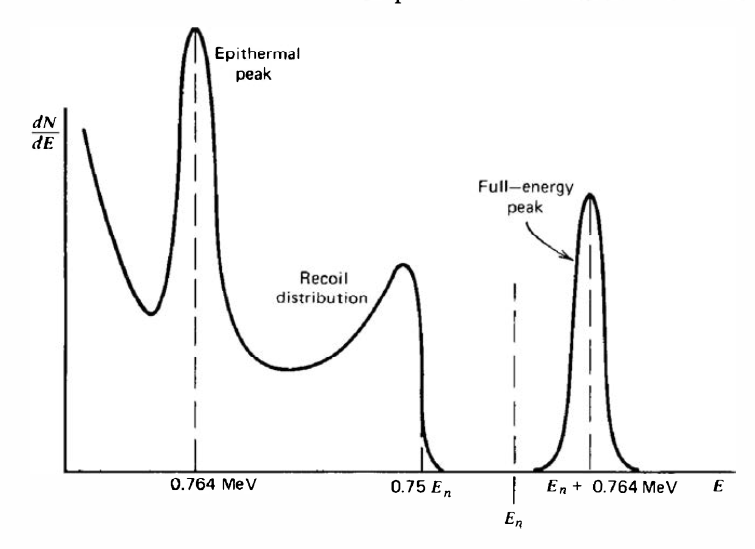
\includegraphics[width=0.7\textwidth]{images/fast_neutrons_3He.png}
    \caption{Idealized fast neutron spectrum from a $^3$He detector.}
    \label{fig:fast_neutrons_3He}
\end{figure}
\begin{itemize}
    \item n $+$ $^3$He $\rightarrow$ p $+$ $^3$H, Q $=$ 764 keV
    \item Ignoring the wall effect, the idealized fast neutron spectrum is shown in figure~\ref{fig:fast_neutrons_3He}. Three distinct features should be seen:
    \begin{enumerate}
        \item The full energy peak corresponding to all the (n,p) reactions induced directly by the incident neutrons. The peak occurs at the energy of the Q-value plus the neutron energy. 
        \item A continuum from elastic scattering of the enutron and a partial transfer of its energy to a recoiling He nucleus. The maximum energy of the continuum can be calculated with the equation of $E_{Rm\text{MAX}}$ given above; it is 75\% of the incoming neutron energy. 
        \item An epithermal peak corresponding to the detection of incident neutrons that have been reduced to the thermal range by moderation in external materials. It occurs at the Q-value. 
    \end{enumerate}
\end{itemize}

\subsubsection{Other Fast Neutron Detectors}
\begin{figure}[ht]
    \centering
    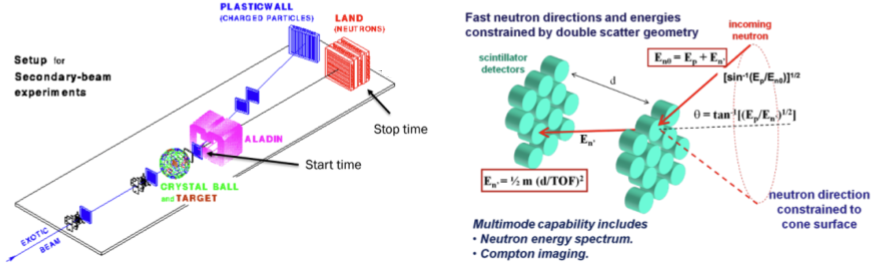
\includegraphics[width=1.0\textwidth]{images/position_fast_neutron.png}
    \caption{GSI-LAND (left) and neutron scatter camera (right).}
    \label{fig:position_fast_neutron}
\end{figure}
\begin{itemize}
    \item Position-sensitive fast neutron detectors (figure~\ref{fig:position_fast_neutron} (left)):\\
    2D array of fast ($\sim$ns decay time) plastic scintillators providing 4$\pi$ coverage to measure neutrons energies via ToF (measurement of time difference between particle tracking detector and neutron detector).
    \item Neutron scatter camera (figure~\ref{fig:position_fast_neutron} (right)):\\
    With liquid, Stilbene, of plastic scintillator arrays or other 3D position-sensitive detectors; neutron-gamma PSD required.
\end{itemize}
\subsubsection{Pulse-Shape Discrimination}
\begin{itemize}
    \item In figure~\ref{fig:organic_scintillator_psd}, we've seen PSD capabilities of organic scintillators. 
    \item With the advantages of being cheap, robust, and of any shape over Stilbene (crystal) and liquid scintillators, plastic scintillators can be used for PSD as well. 
    \item $^6$Li can be added for thermal neutron detection.
    \item Figure~\ref{fig:decay_time_plastic_scintillator} and figure~\ref{fig:PSD_plastic_scintillator} show the PSD capabilities of plastic scintillators.
\end{itemize}
\begin{figure}[ht]
    \centering
    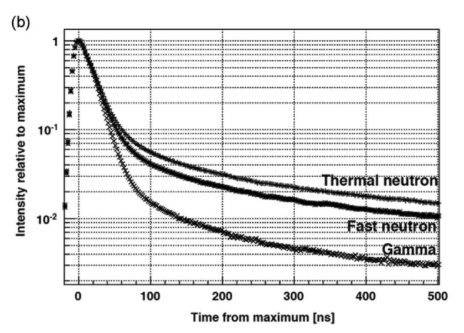
\includegraphics[width=0.4\textwidth]{images/decay_time_plastic_scintillator.png}
    \caption{Decay time dependence on particle type in plastic scintillators.}
    \label{fig:decay_time_plastic_scintillator}
\end{figure}
\begin{figure}[ht]
    \centering
    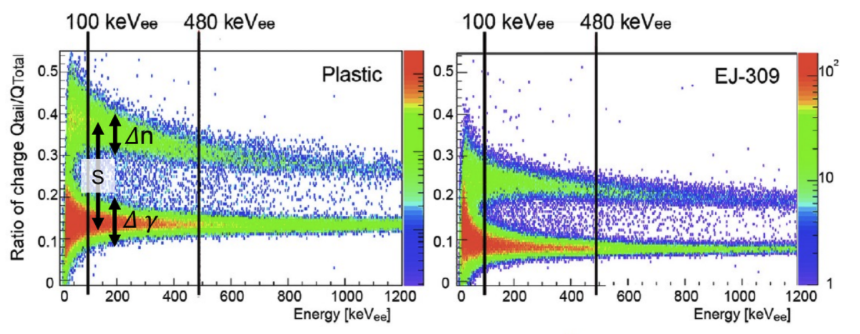
\includegraphics[width=0.8\textwidth]{images/PSD_plastic_scintillator.png}
    \caption{PSD in plastic scintillators (left) and liquid scintillators (right). Figure-of-merit given by $S/(\Delta n+\Delta\gamma)$.}
    \label{fig:PSD_plastic_scintillator}
\end{figure}
\subsection{Miscellaneous Neutron Detectors}
\subsubsection{Nuclear Reactor Instrumentation}
\begin{itemize}
    \item Thermal neutron detection capabilities (obviously) required
    \item Detection systems have to withstand extreme heat and pressure, high radiation fields (neutron and gammas), and provide long-term stability and a large range of sensitivity.
    \item There are 2 categories of detection systems:
    \begin{enumerate}
        \item In-core, current mode:
        \begin{itemize}
            \item Located within narrow coolant channels in the core to provide flux shape within the core
            \item Rate of $>10^7$ 1/s, up to rates causing unacceptable recombination effects
            \item No discrimination against gammas, except signal amplitude current fluctuations (Campbelling technique of fission counters)
            \item Compensated ionization chambers (CIC) can be used to subtract the gamma-ray signal component, with the setup shown in figure~\ref{fig:compensated_ion_chamber}. 
            \item Self-powered detectors (SPD) can directly measure currents due to beta electrons or gamma-induced electrons without an external applied voltage.
            \item Fission chambers can be tailored for any power range. They are small, $^{235}$U-line Ar-filled gas detectors, with fertile $^{234}$U added to increase longevity (regenerative chambers). Buildup of fission products within the chamber, which contributes significantly to current signals, leads to memory effects. 
        \end{itemize}
        \begin{figure}[ht]
            \centering
            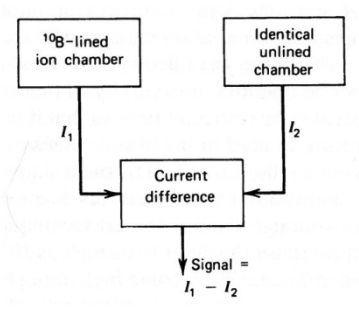
\includegraphics[width=0.35\textwidth]{images/compensated_ion_chamber.png}
            \caption{Configuration of a compensated ionization chamber. The boron-lined ion chamber is sensitive to both neutrons and gammas, and the chamber without boron lining is sensitive to only gammas. The difference in the currents gives the neutron-only component.}
            \label{fig:compensated_ion_chamber}
        \end{figure}
        \item Out-of-core, pulse-mode:
        \begin{itemize}
            \item Located outside the core to provide integrated neutron flux over the entire core
            \item Rate $<10^5\sim10^7$ 1/s
            \item Proportional detectors with $\gamma$-discrimination
        \end{itemize}
    \end{enumerate}
\end{itemize}